\section{Jordan Measure} %

% --- TEACHER'S INTRO ---
\begin{extra}
\textbf{Teacher's Note: The \qt{Pixel} Approach to Area}\\
Before we look at the formal math, let's think about computer screens. How does a computer display a circle? It uses pixels! If the pixels are huge, the circle looks like a blocky mess. If the pixels are tiny, it looks perfectly smooth. 

Jordan measure is exactly this idea. We want to find the volume of strange, curvy shapes by approximating them with blocky \qt{pixels} (which we call \qt{dyadic cubes}). 
\begin{itemize}
    \item If we take all the pixels that touch the shape (even a little bit), we get an \qt{outer approximation} (an overestimate).
    \item If we only take the pixels that are $100\%$ inside the shape, we get an \qt{inner approximation} (an underestimate).
\end{itemize}
If we make our pixels infinitely small, and the inner and outer approximations squeeze together to the exact same number, we say the shape is \qt{Jordan measurable}!
\end{extra}
% -----------------------

\subsection{Dyadic Cubes: Intuition vs. Script}

To build our grid, we use a very specific type of building block. Here is how your TA intuitively described it:

\begin{definition*}[TA's Intuitive Dyadic Cubes] %
A \qt{dyadic cube} of side length $2^{-p}$ (for some integer $p \ge 0$) is defined on a standard coordinate grid. The union of finite, same-size dyadic cubes is called a \qt{dyadic set}. %

For a fixed \qt{pixel size} $2^{-p}$, a dyadic set $E$ in $\mathbb{R}^n$ can be represented mathematically as: %
\[
E = \bigcup_{l=1}^N 2^{-p}\left(a(l) + [0,1)^n\right), %
\]
where $a(l) \in \mathbb{Z}^n$ is an integer vector representing the coordinates of the bottom-left corner of each cube in the grid. %
\end{definition*}

% --- TEACHER'S VISUALIZATION: DYADIC SUBDIVISION ---
\begin{center}
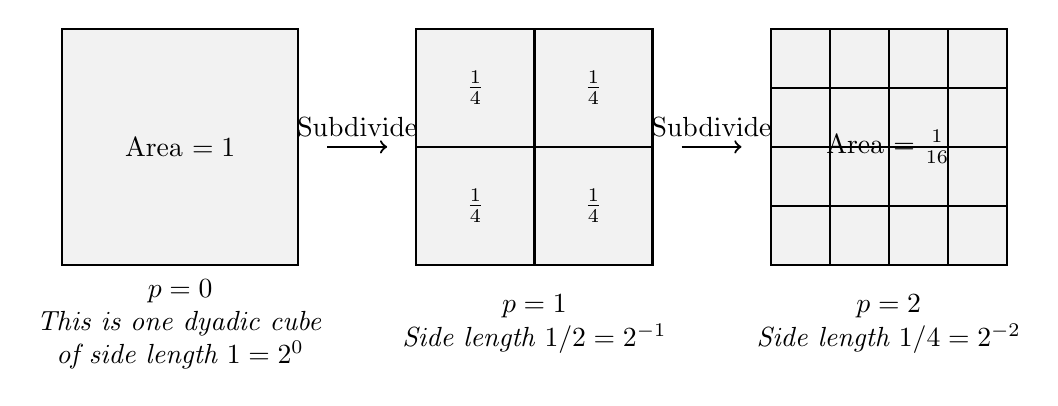
\begin{tikzpicture}[scale=1.5]
    % Level 0 (p=0)
    \begin{scope}[xshift=0cm]
        \draw[thick, fill=gray!10] (0,0) rectangle (2,2);
        \node[align=center] at (1, -0.5) {$p=0$ \\ \textit{This is one dyadic cube} \\ \textit{of side length $1 = 2^0$}};
        \node at (1, 1) {Area $= 1$};
    \end{scope}

    % Arrow
    \draw[->, thick, shorten >=2pt, shorten <=2pt] (2.2, 1) -- (2.8, 1) node[midway, above] {Subdivide};

    % Level 1 (p=1)
    \begin{scope}[xshift=3cm]
        \draw[thick, fill=gray!10] (0,0) rectangle (2,2);
        \draw[thick] (1,0) -- (1,2);
        \draw[thick] (0,1) -- (2,1);
        \node[align=center] at (1, -0.5) {$p=1$ \\ \textit{Side length $1/2 = 2^{-1}$}};
        \node at (0.5, 0.5) {$\frac{1}{4}$};
        \node at (1.5, 0.5) {$\frac{1}{4}$};
        \node at (0.5, 1.5) {$\frac{1}{4}$};
        \node at (1.5, 1.5) {$\frac{1}{4}$};
    \end{scope}

    % Arrow
    \draw[->, thick, shorten >=2pt, shorten <=2pt] (5.2, 1) -- (5.8, 1) node[midway, above] {Subdivide};

    % Level 2 (p=2)
    \begin{scope}[xshift=6cm]
        \draw[thick, fill=gray!10] (0,0) rectangle (2,2);
        \draw[step=0.5, thick] (0,0) grid (2,2);
        \node[align=center] at (1, -0.5) {$p=2$ \\ \textit{Side length $1/4 = 2^{-2}$}};
        \node at (1, 1) {Area $= \frac{1}{16}$};
    \end{scope}
\end{tikzpicture}
\end{center}
\vspace{0.5cm}
% ----------------------------------------------------

Any dyadic cube can be perfectly subdivided into smaller cubes. If we want to compare two different dyadic sets that have different pixel sizes, we can always choose the smallest pixel size and subdivide the larger cubes to match. 

Now, let's look at the rigorous definition from the official script:

% --- SCRIPT COUNTERS SETUP ---
% Save current counters
\newcounter{savedSectionJM}
\setcounter{savedSectionJM}{\value{section}}
\newcounter{savedDefJM}
\setcounter{savedDefJM}{\value{theorem}}

% Set counters to exactly match the script (Section 13, Definition 13.1)
\setcounter{section}{13}
\setcounter{theorem}{0} 

\begin{definition}[Dyadic Cubes]
A \qt{dyadic cube} of side length $2^{-p}$ ($p \in \mathbb{N}_0$) in $\mathbb{R}^n$ is a set of the form
\[
Q = 2^{-p}(a + [0, 1)^n),
\]
where $a \in \mathbb{Z}^n$. We denote the set of all dyadic cubes of side length $2^{-p}$ by $\Omega_p$.
\end{definition}

\begin{extra}
\textbf{Why half-open intervals $[0,1)^n$?} \\
You might wonder why the definition uses a bracket and a parenthesis. If we used closed intervals $[0,1] \times [0,1]$ for our cubes, their boundaries would overlap. For example, the right edge of the left cube would be the exact same line as the left edge of the right cube. 

By defining them as $[0,1)$, we mean \qt{include the left and bottom edges, but leave the top and right edges open}. This ensures that every single point in $\mathbb{R}^n$ belongs to exactly \textit{one} unique dyadic cube. No double counting!
\end{extra}


\subsection{Inner and Outer Volumes}

Similar to the Riemann Integral in 1D, we define the volume (measure) of an arbitrary set $A \subset \mathbb{R}^n$ by approximating it from the outside and from the inside. First, note that the volume (or measure $\mu$) of a single dyadic cube in $\mathbb{R}^n$ at level $p$ is simply $\mu(Q) = 2^{-pn}$. %

Here is the rigorous script definition for these approximations:

% Counter is already at 13.1, so the next definition will be 13.2
\begin{definition}[Inner and Outer Approximations]
Let $A \subset \mathbb{R}^n$ be a bounded set. For $p \in \mathbb{N}_0$, we define the \textbf{inner approximation} $I(A, p)$ and the \textbf{outer approximation} $O(A, p)$ by:
\begin{align*}
I(A, p) &:= \bigcup \{ Q \in \Omega_p \mid \overline{Q} \subset A^\circ \}, \\
O(A, p) &:= \bigcup \{ Q \in \Omega_p \mid Q \cap A \neq \emptyset \}.
\end{align*}
Here, $\overline{Q}$ is the closure of the cube, and $A^\circ$ is the interior of $A$. 
\end{definition}

\begin{definition}[Jordan Measure]
The \textbf{inner measure} and \textbf{outer measure} of $A$ are defined as the limits of the volumes of these approximations:
\[
\mu_{\text{in}}(A) := \lim_{p \to \infty} \mu(I(A, p)), \quad \text{and} \quad \mu_{\text{out}}(A) := \lim_{p \to \infty} \mu(O(A, p)).
\]
A bounded set $A \subset \mathbb{R}^n$ is called \textbf{Jordan measurable} if $\mu_{\text{in}}(A) = \mu_{\text{out}}(A)$. In this case, this common value is called the Jordan measure of $A$, denoted by $\mu(A)$.
\end{definition}

% --- RESTORE COUNTERS ---
\setcounter{section}{\value{savedSectionJM}}
\setcounter{theorem}{\value{savedDefJM}}

\begin{extra}
\textbf{Teacher's Note: Bridging the Script to the TA Notes}\\
Wow, the script's definition looks scary! But it is exactly what we drew in the TA notes (where the TA used $F_i$ for inner and $G_i$ for outer approximations). 
\begin{itemize}
    \item The script's $p$ (level of subdivision) is just the TA's index $i$.
    \item The script's $O(A,p)$ is the TA's $G_i$. The condition $Q \cap A \neq \emptyset$ literally just means \qt{include the cube if it touches the set A at all.}
    \item The script's $I(A,p)$ is the TA's $F_i$. The condition $\overline{Q} \subset A^\circ$ is just a rigorous topological way of saying \qt{the cube must be 100\% safely inside the boundaries of A.}
\end{itemize}
So whenever you see $I(A,p)$ and $O(A,p)$ on the exam, just picture the blue and red pixel grids below!
\end{extra}


% --- TEACHER'S VISUALIZATION: OUTER SEQUENCE ---
\begin{center}
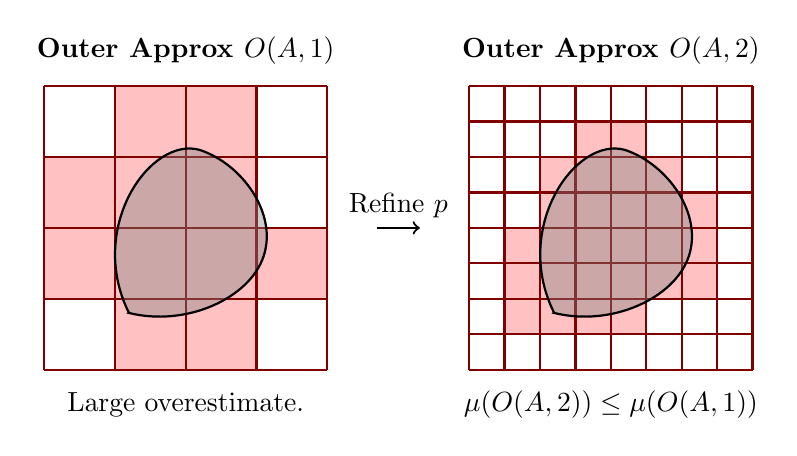
\begin{tikzpicture}[scale=0.9]
    % --- LEFT PANEL: OUTER 1 ---
    \begin{scope}[xshift=0cm]
        \node at (2, 4.5) {\textbf{Outer Approx $O(A, 1)$}};
        
        \draw[step=1.0, gray!30, thin] (0,0) grid (4,4);
        
        % Fill Outer 1
        \fill[red!30, opacity=0.8] 
            (1,0) rectangle (3,1)
            (0,1) rectangle (4,2)
            (0,2) rectangle (3,3)
            (1,3) rectangle (3,4);
            
        \draw[step=1.0, red!50!black, thick] (0,0) grid (4,4);
        
        % The Blob
        \draw[thick, black, fill=gray, fill opacity=0.4] 
            (1.2, 0.8) .. controls (0.6, 2.0) and (1.5, 3.3) .. 
            (2.2, 3.1) .. controls (2.8, 2.9) and (3.3, 2.2) .. 
            (3.1, 1.6) .. controls (2.9, 1.0) and (2.0, 0.6) .. cycle;
            
        \node at (2, -0.5) {Large overestimate.};
    \end{scope}

    \draw[->, thick, shorten >=5pt, shorten <=5pt] (4.5, 2) -- (5.5, 2) node[midway, above] {Refine $p$};

    % --- RIGHT PANEL: OUTER 2 ---
    \begin{scope}[xshift=6cm]
        \node at (2, 4.5) {\textbf{Outer Approx $O(A, 2)$}};
        
        \draw[step=0.5, gray!30, thin] (0,0) grid (4,4);
        
        % Fill Outer 2 
        \fill[red!30, opacity=0.8] 
            (0.5, 0.5) rectangle (2.5, 1.0)
            (0.5, 1.0) rectangle (3.5, 1.5)
            (0.5, 1.5) rectangle (3.5, 2.0)
            (1.0, 2.0) rectangle (3.5, 2.5)
            (1.0, 2.5) rectangle (3.0, 3.0)
            (1.5, 3.0) rectangle (2.5, 3.5);
            
        \draw[step=0.5, red!50!black, thick] (0,0) grid (4,4);
        
        % The Blob
        \draw[thick, black, fill=gray, fill opacity=0.4] 
            (1.2, 0.8) .. controls (0.6, 2.0) and (1.5, 3.3) .. 
            (2.2, 3.1) .. controls (2.8, 2.9) and (3.3, 2.2) .. 
            (3.1, 1.6) .. controls (2.9, 1.0) and (2.0, 0.6) .. cycle;
            
        \node at (2, -0.5) {$\mu(O(A, 2)) \le \mu(O(A, 1))$};
    \end{scope}
\end{tikzpicture}
\end{center}
\vspace{0.5cm}
% --------------------------------------------------------

% --- TEACHER'S VISUALIZATION: INNER SEQUENCE ---
\begin{center}
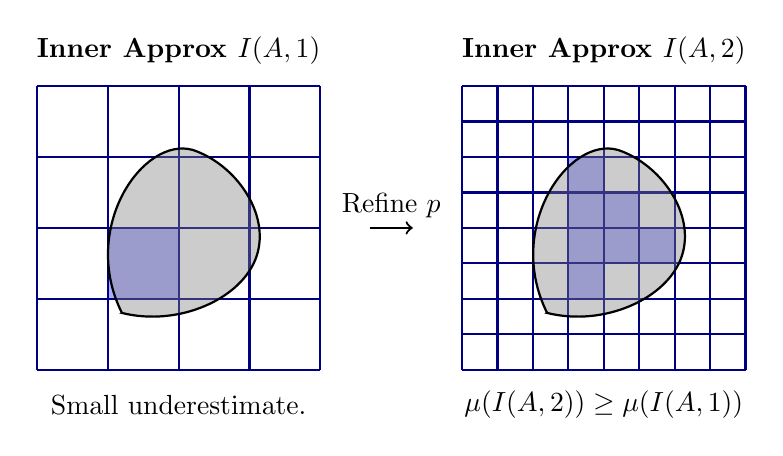
\begin{tikzpicture}[scale=0.9]
    % --- LEFT PANEL: INNER 1 ---
    \begin{scope}[xshift=0cm]
        \node at (2, 4.5) {\textbf{Inner Approx $I(A, 1)$}};
        
        \draw[step=1.0, gray!30, thin] (0,0) grid (4,4);
        
        % Fill Inner 1
        \fill[blue!40, opacity=0.8] 
            (1,1) rectangle (2,2);
            
        \draw[step=1.0, blue!50!black, thick] (0,0) grid (4,4);
        
        % The Blob
        \draw[thick, black, fill=gray, fill opacity=0.4] 
            (1.2, 0.8) .. controls (0.6, 2.0) and (1.5, 3.3) .. 
            (2.2, 3.1) .. controls (2.8, 2.9) and (3.3, 2.2) .. 
            (3.1, 1.6) .. controls (2.9, 1.0) and (2.0, 0.6) .. cycle;
            
        \node at (2, -0.5) {Small underestimate.};
    \end{scope}

    \draw[->, thick, shorten >=5pt, shorten <=5pt] (4.5, 2) -- (5.5, 2) node[midway, above] {Refine $p$};

    % --- RIGHT PANEL: INNER 2 ---
    \begin{scope}[xshift=6cm]
        \node at (2, 4.5) {\textbf{Inner Approx $I(A, 2)$}};
        
        \draw[step=0.5, gray!30, thin] (0,0) grid (4,4);
        
        % Fill Inner 2
        \fill[blue!40, opacity=0.8] 
            (1.5, 1.0) rectangle (2.0, 1.5)
            (1.5, 1.5) rectangle (2.0, 2.0)
            (2.0, 1.5) rectangle (2.5, 2.0)
            (2.5, 1.5) rectangle (3.0, 2.0)
            (1.5, 2.0) rectangle (2.0, 2.5)
            (2.0, 2.0) rectangle (2.5, 2.5)
            (1.5, 2.5) rectangle (2.0, 3.0);
            
        \draw[step=0.5, blue!50!black, thick] (0,0) grid (4,4);
        
        % The Blob
        \draw[thick, black, fill=gray, fill opacity=0.4] 
            (1.2, 0.8) .. controls (0.6, 2.0) and (1.5, 3.3) .. 
            (2.2, 3.1) .. controls (2.8, 2.9) and (3.3, 2.2) .. 
            (3.1, 1.6) .. controls (2.9, 1.0) and (2.0, 0.6) .. cycle;
            
        \node at (2, -0.5) {$\mu(I(A, 2)) \ge \mu(I(A, 1))$};
    \end{scope}
\end{tikzpicture}
\end{center}